%\section{Fully Rational vs. Behavioral Best-Responses by Agents}\label{sec:agetns-response}
\section{Agents' Strategic Responses}\label{sec:agetns-response}

\begin{figure*}[t]
    \centering
    \begin{subfigure}[t]{0.3\textwidth}
        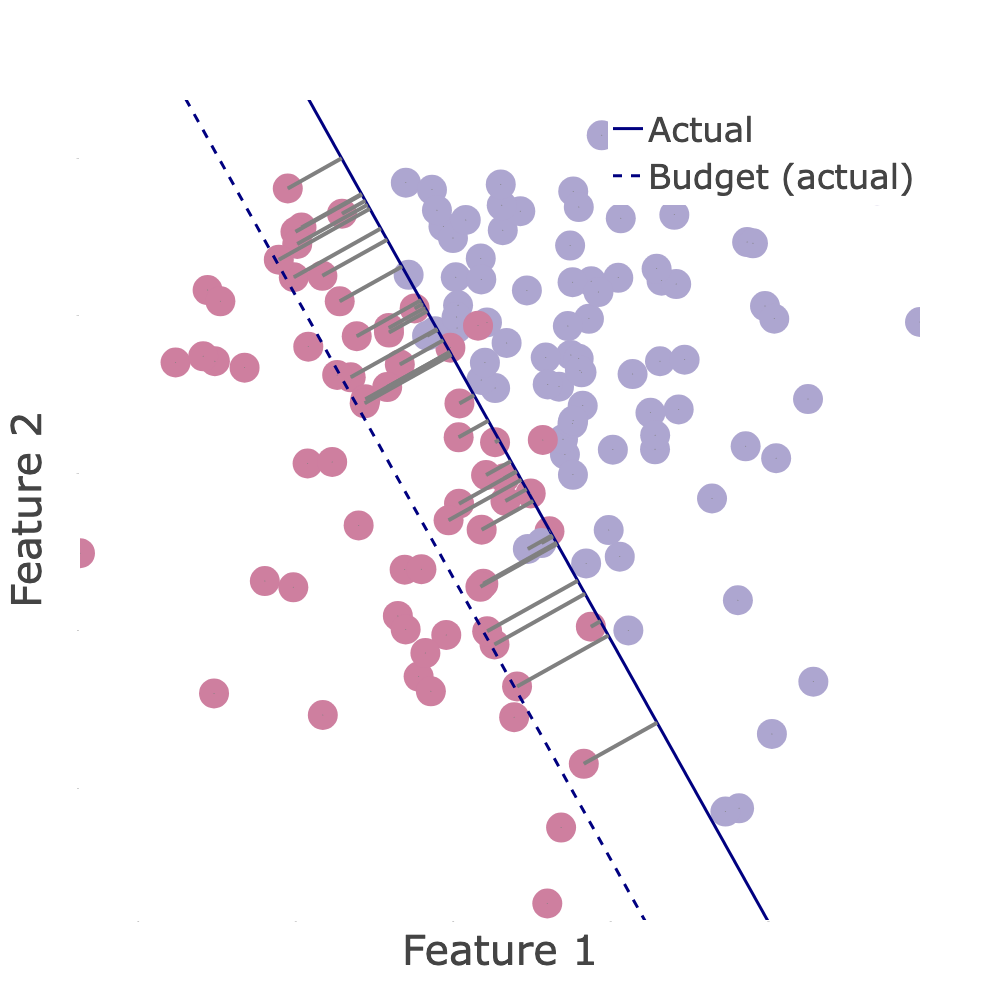
\includegraphics[width=0.82\textwidth]{Figures/NB_movement_arrows.png}
            \caption{Rational strategic response}
            \Description[Rational strategic response]{This figure shows the rational response of agents to a known threshold classifier in 2 dimensions.}
        \label{fig:NB-arrows}
    \end{subfigure}
    \begin{subfigure}[t]{0.3\textwidth}
        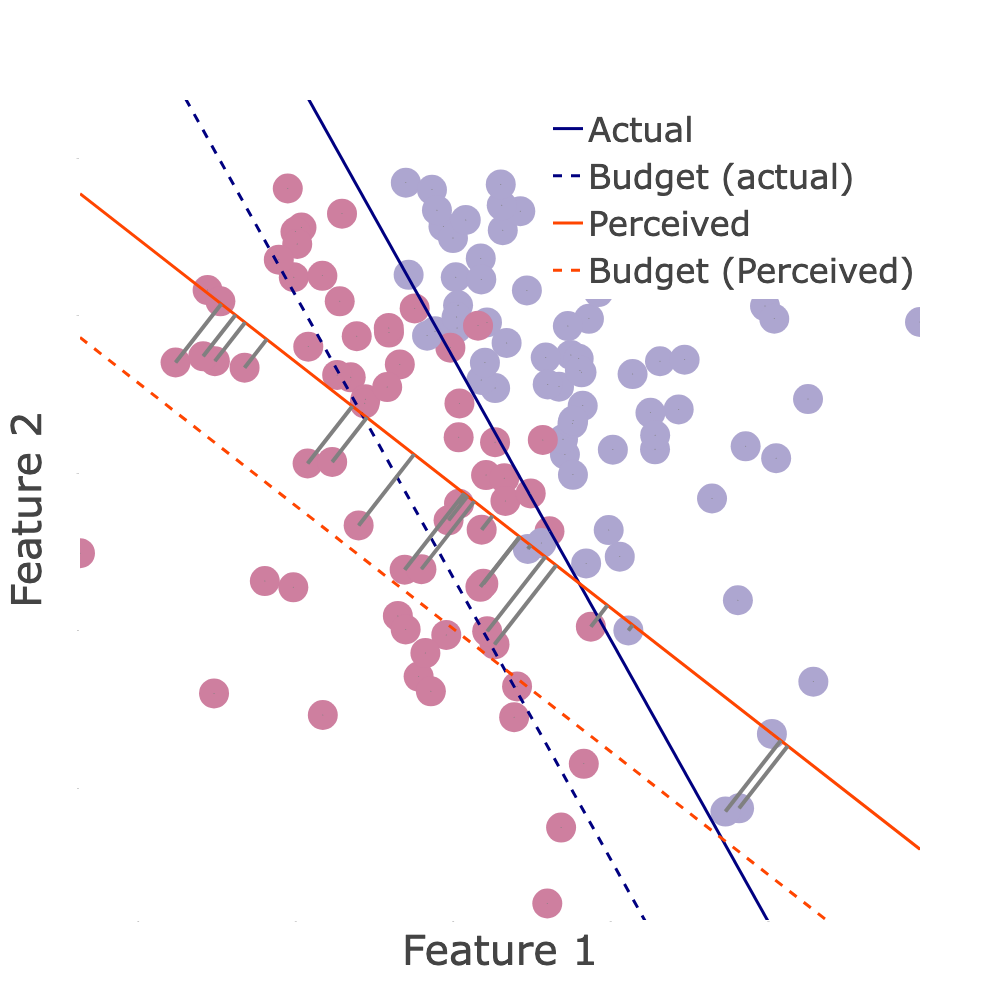
\includegraphics[width=0.82\textwidth]{Figures/B_movement_arrows.png}
        \caption{Biased strategic response}
        \Description[Biased strategic response]{This figure shows the biased response of agents to a known threshold classifier in 2 dimensions.}
        \label{fig:B-arrows}
    \end{subfigure}
    \hspace{0.01in}
    \begin{subfigure}[t]{0.3\textwidth}
        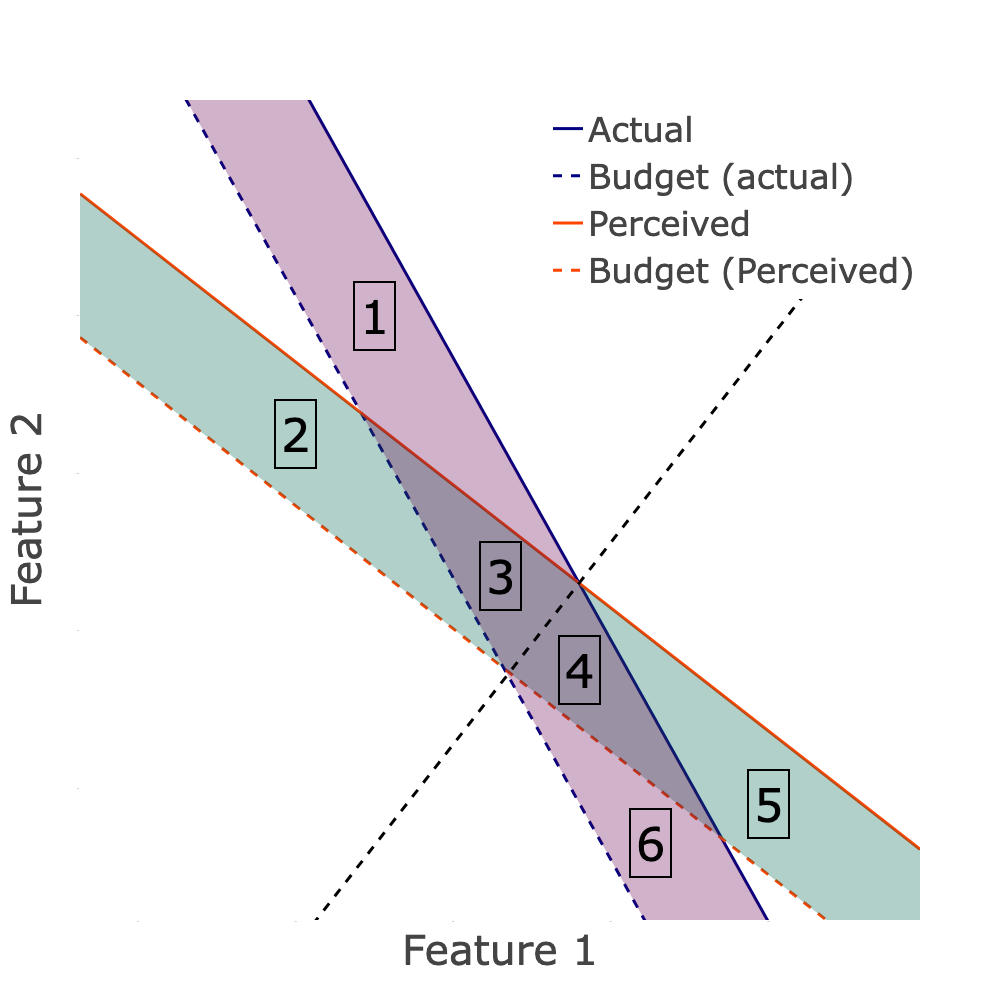
\includegraphics[width=0.82\textwidth]{Figures/B_highlighted_regions.png}
            \caption{Differing strategic responses}
            \Description[Differing strategic response]{This figure shows the regions for the differences between the response of biased and rational agents to a known threshold classifier in 2 dimensions.}
        \label{fig:highlighted}
    \end{subfigure}
    \caption{(a) Fully rational responses, (b) Behaviorally biased responses, and (c) Classes of differing actions. (norm-2 costs)}
    \Description[Rational and biased strategic response]{This figure shows an example of biased and rational response to an algorithm in 2 dimensions.}
    \label{fig:BR-illustration}
\end{figure*} 

We first fix the classifier $(\vtheta, \theta_0)$, and compare fully rational (non-behavioral) and behavioral agents' strategic responses to it. The following Lemma characterizes $\vx_\text{NB}$ (the solution to the optimization problem in \eqref{eq:agent-optimization}) and $\vx_\text{B}$ (the solution to the optimization problem in \eqref{eq:agent-optimization-behavioral}) under the norm-2 cost. All proofs are included in Appendix~\ref{sec:app-proofs}. 


\begin{lemma}\label{lemma:band-optimization}
    Let $d(\vx_0, \vtheta, \theta_0)=\frac{\theta_0-\vtheta^T\vx_0}{\norm{\vtheta}_2^2}$  denote $\vx_0$'s distance to the hyperplane $\vtheta^T\vx=\theta_0$. Then, for an agent with starting feature vector $\vx_0$, if $0 < d(\vx_0, \vtheta, \theta_{0}) \le B$, 
    \begin{align*}
        \vx_\text{NB} = \vx_0 + d(\vx_0, \vtheta, \theta_{0})\vtheta~.%\\
    \end{align*}
    Otherwise, $\vx_\text{NB} = \vx_0$. For behaviorally biased agents, $\vx_{B}$ is obtained similarly by replacing $\vtheta$ with $\vw(\vtheta)$.
\end{lemma}

Figure~\ref{fig:BR-illustration} illustrates the strategic agents' best-responses of Lemma~\ref{lemma:band-optimization}, in a two-dimensional feature space, when they are non-behavioral (Fig.~\ref{fig:NB-arrows}) and when they are behavioral (Fig.~\ref{fig:B-arrows}). We first note that the subset of agents with non-trivial responses to the classifier, as identified in  Lemma~\ref{lemma:band-optimization}, are in a band below the decision boundary. Given the overlaps of these bands under non-behavioral and behavioral responses, there are 6 regions of interest where biased agents' best-responses differ from rational agents (Fig.~\ref{fig:highlighted}). In regions \framebox(7,9){1} and \framebox(7,9){6}, agents invest no effort in manipulating their features when they are behaviorally biased, whereas they do when fully rational; the reasons differ: agents in \framebox(7,9){1} believe they are accepted without effort, while those in \framebox(7,9){6} believe they do not have sufficient budget to succeed. Agents in regions \framebox(7,9){2} and \framebox(7,9){5} manipulate their features unnecessarily (they would not, had they been fully rational), and again, for different reasons: agents in \framebox(7,9){2} are not accepted even at their highest effort level, while those in \framebox(7,9){5} believe they must reach the boundary but they would be accepted regardless of their effort. Finally, in region \framebox(7,9){3}, agents \emph{undershoot} the actual boundary (i.e., exert less effort than needed due to their biases), while those in region \framebox(7,9){4} \emph{overshoot} (i.e., exert more effort than needed to get accepted). 


In the following proposition, we further investigate best-responses in region \framebox(7,9){4} (resp. region \framebox(7,9){3}) and identify which features behavioral agents over-invest in (resp. under-invest in) that leads to them overshooting (resp. undershooting) past the true classifier $(\vtheta, \theta_0)$. 
\begin{proposition}\label{prop:under-invest-high-dim}
Consider an agent with features $\vx_0$, facing classifier $(\vtheta, \theta_0)$, and with a misperceived $\vw(\vtheta)$. Let $\theta_{\max}=\max_i \theta_i$, $d(\vx_0, \vtheta, \theta_0)=\frac{\theta_0-\vtheta^T\vx_0}{\norm{\vtheta}_2^2}$, and  $\delta^{\text{NB}}_i=x_{\text{NB},i}-x_{0,i}$ and $\delta^{\text{B}}_i=x_{\text{B},i}-x_{0,i}$ denote the changes in feature $i$ after best-responses. Then:\\[2pt]
    \hspace*{0.1in}{\textbf{(1)}} If $d(\vx_0, \vw(\vtheta), \theta_0)\le d(\vx_0, \vtheta, \theta_0)$ and $w(\theta_i)<\theta_i$, then $\delta_i^{\text{B}}<\delta_i^{\text{NB}}$.\\[2pt]
    \hspace*{0.1in}\textbf{(2)} If $d(\vx_0, \vtheta, \theta_0)\le d(\vx_0, \vw(\vtheta), \theta_0)$ and $\theta_i<w(\theta_i)$ then $\delta_i^{\text{NB}}<\delta_i^{\text{B}}$.\\[2pt]
    \hspace*{0.1in}\textbf{(3)} For the special case of a Prelec function, we further have: If $d(\vx_0, \vtheta, \theta_0) \le e^{\gamma^\frac{1}{1-\gamma}-\gamma^\frac{\gamma}{1-\gamma}} d(\vx_0, \vw(\vtheta), \theta_0)$ and $w(\theta_{\max})<\theta_{\max}$, then
    $\delta_{\max}^{\text{NB}}<\delta_{\max}^{\text{B}}$. 
\end{proposition}

Intuitively, the proposition states that agents who perceive the decision boundary to be closer to them than it truly is (regions \framebox(7, 9){2} and \framebox(7, 9){3} in Figure~\ref{fig:highlighted}) will under-invest in the features for which they underestimate the importance. Similarly, agents that perceive the boundary to be farther (regions \framebox(7, 9){4} and \framebox(7, 9){5} in Figure~\ref{fig:highlighted}) will over-invest in the features for which they overestimate the importance. 
